\comment{Suggestion: past tense}\\

\subsection{Gradient Descent Analysis}
    
    \subsubsection{OLS Optimisation}
        All plots regarding the optimisation of the OLS cost function are found in \cref{res:fig:lrates}.

        \begin{table}[!ht]
            \centering
            \begin{tabular}{r|c|l}
                Method & MSE & $\eta$ \\ \hline
                Plain GD & 0.2522 & 0.0719 \\
                Momentum GD & 0.1738 & 0.132 \\
                Plain SGD & 0.1827 & 0.0622 \\
                Momentum SGD & 0.1719 & 0.0914 \\
                AdaGrad GD & 0.2725 & 0.525 \\
                AdaGrad Momentum GD & 0.2065 & 0.567 \\
                AdaGrad SGD & 0.2017 & 0.546 \\
                AdaGrad Momentum SGD & 0.1762 & 0.651 \\
                RMSprop SGD & 0.1778 & 0.277 \\
                Adam SGD & 0.1736 & 0.287 \\
            \end{tabular}
            \caption{Table of the best validation MSE scores by GD algorithm, together with the learning rate that produced the best result.}
            \label[tab]{res:tab:OLS_MSEs}
        \end{table}

    \begin{figure*}
        \begin{subfigure}{.5\textwidth}
            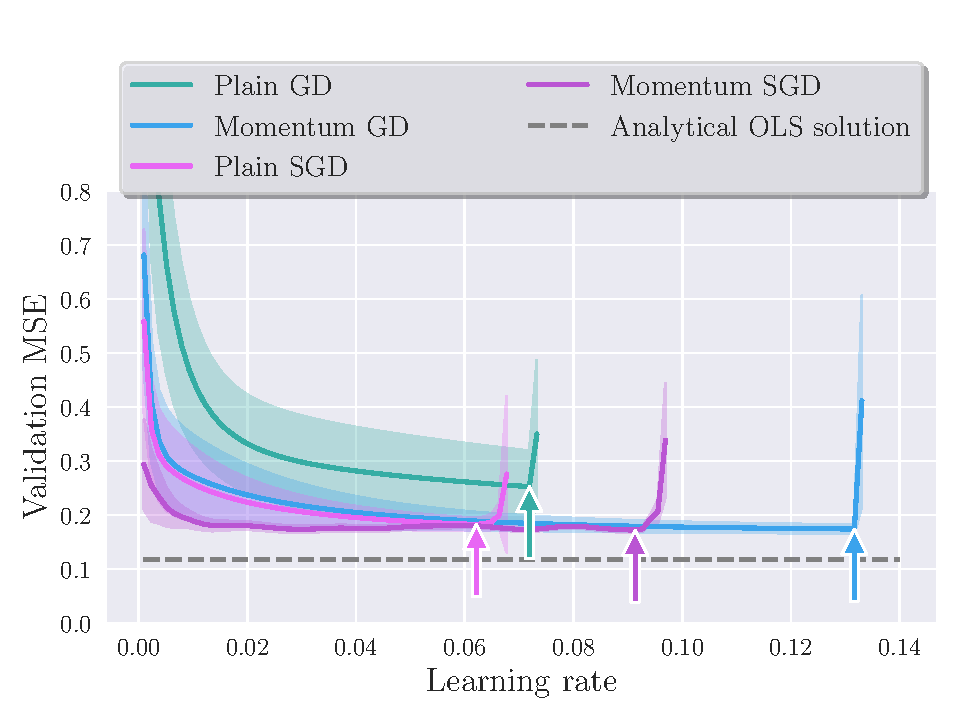
\includegraphics[width=\linewidth]{learning_rates_PGD_MGD_PSGD_MSGD.pdf}
            \caption{Best MSEs, learning rates: (0.2522, 0.0719), (0.1738, 0.132), (0.1787, 0.0399), (0.1755, 0.00934)}
            \label[fig]{res:fig:lrate1}
        \end{subfigure}
        \hfill
        \begin{subfigure}{.5\textwidth}
            \centering
            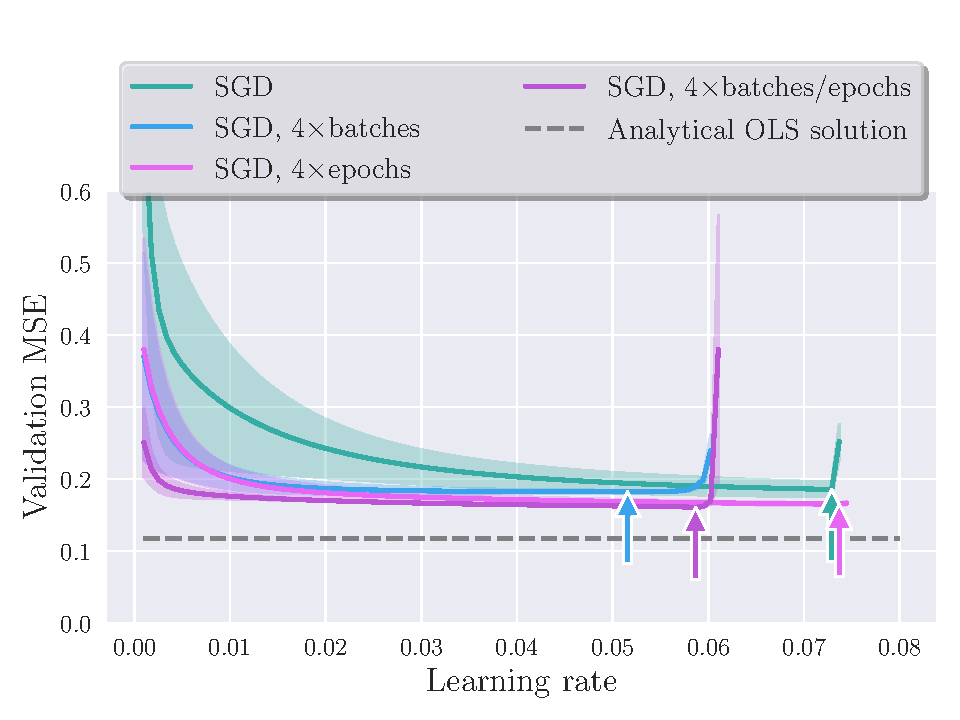
\includegraphics[width=\linewidth]{learning_rates_SGD_batches_epochs.pdf}
            \caption{Best MSEs, learning rates: (0.1827, 0.0618), (0.1807, 0.0279), (0.1667, 0.0539), (0.1767, 0.0168)}
            \label[fig]{res:fig:lrate2}
        \end{subfigure}
        \hfill
        \begin{subfigure}{.5\textwidth}
            \centering
            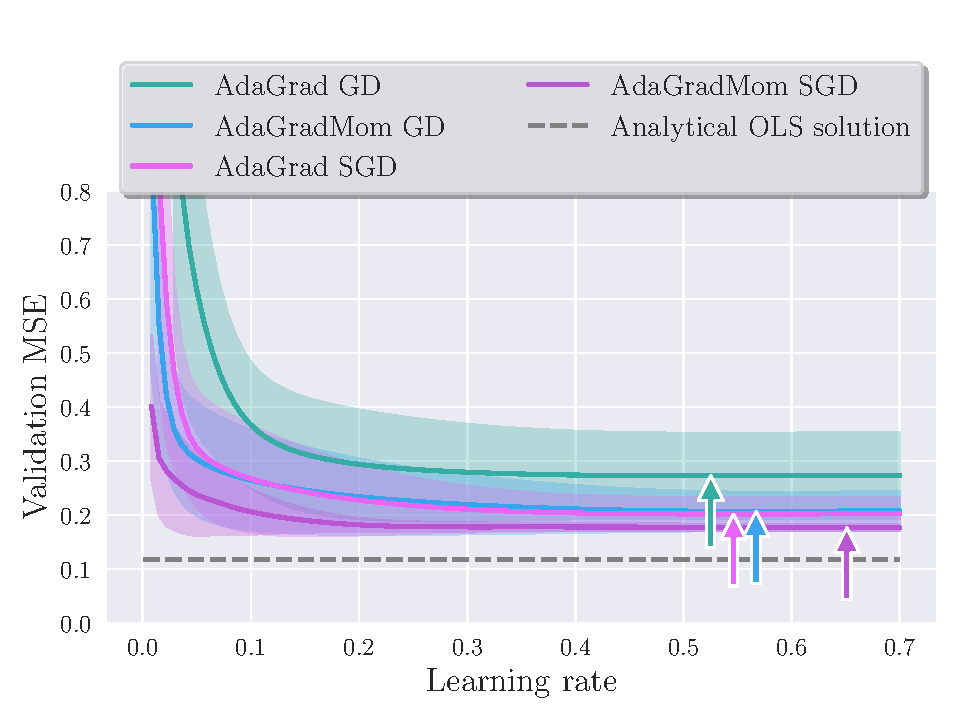
\includegraphics[width=\linewidth]{learning_rates_adagrad}
            \caption{Best MSEs, learning rates: (0.2725, 0.528), (0.2065, 0.570), (0.1810, 0.576), (0.1784, 0.175)}
            \label[fig]{res:fig:lrate3}
        \end{subfigure}
        \hfill
        \begin{subfigure}{.5\textwidth}
            \centering
            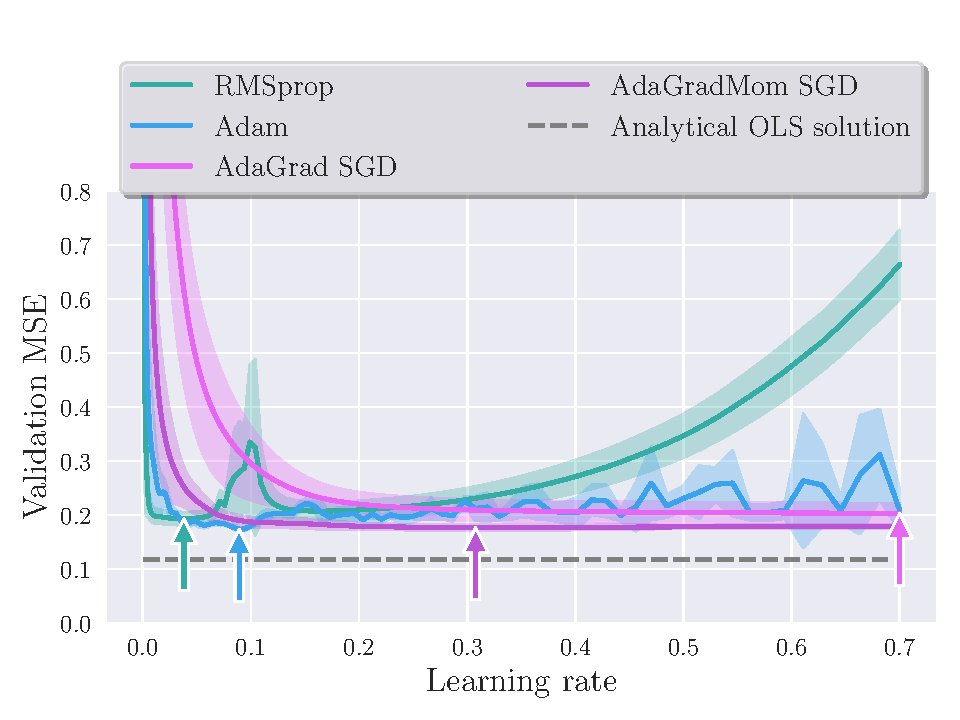
\includegraphics[width=\linewidth]{learning_rates_tunable}
            \caption{Best MSEs, learning rates: (0.1810, 0.569), (0.1784, 0.170), (0.1826, 0.00677), (0.1790, 0.0168)}
            \label[fig]{res:fig:lrate4}
        \end{subfigure}
        \caption{Plots of the validation MSE of the parameters found from optimising the OLS cost function on Franke function data with $n=600$ data points. For the momentum methods we used $\gamma=0.8$. The stochastic methods used a batch size of 64 and 100 epochs, while the standard GD did 100 iterations unless specified otherwise. Overlaid are 95\% confidence intervals based on optimising with five different starting points.
        Analytical OLS MSE: 0.1176.}
        \label[fig]{res:fig:lrates}
    \end{figure*}

\subsection{Wisconsin Breast Cancer}
    \begin{figure*}
        \begin{subfigure}{.5\textwidth}
            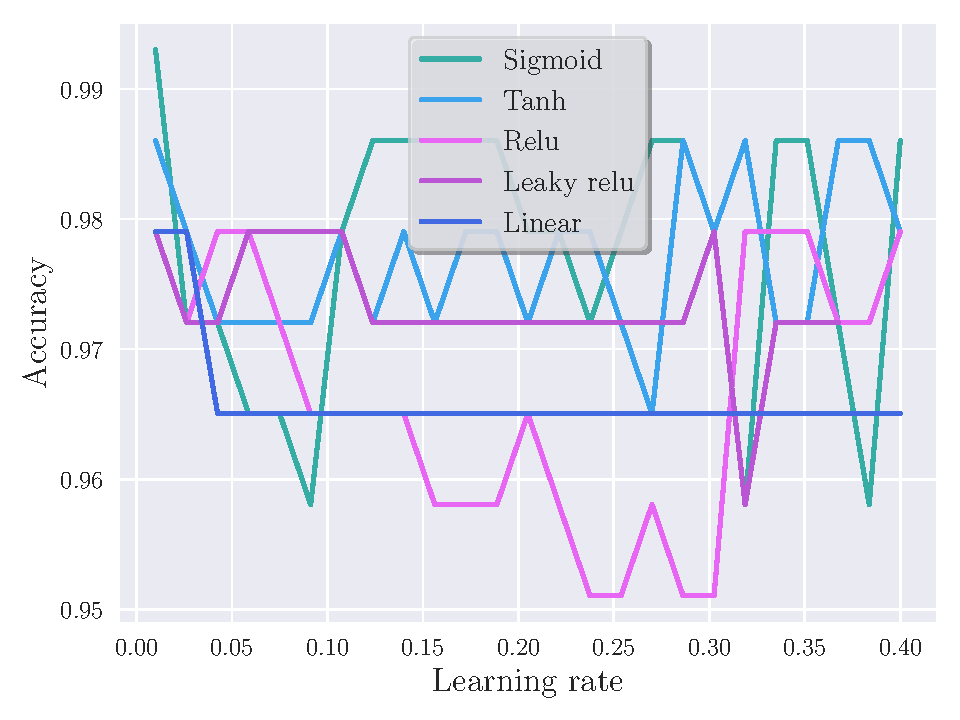
\includegraphics[width=\linewidth]{clasf_activation_functions1.pdf}
            \caption{$\eta \in [ 0.01, 0.4 ]$ with $n = 50$ points. One hidden layer with a single node}
            \label[fig]{res:fig:a}
        \end{subfigure}
        \hfill 
        \begin{subfigure}{.5\textwidth}
            \centering
            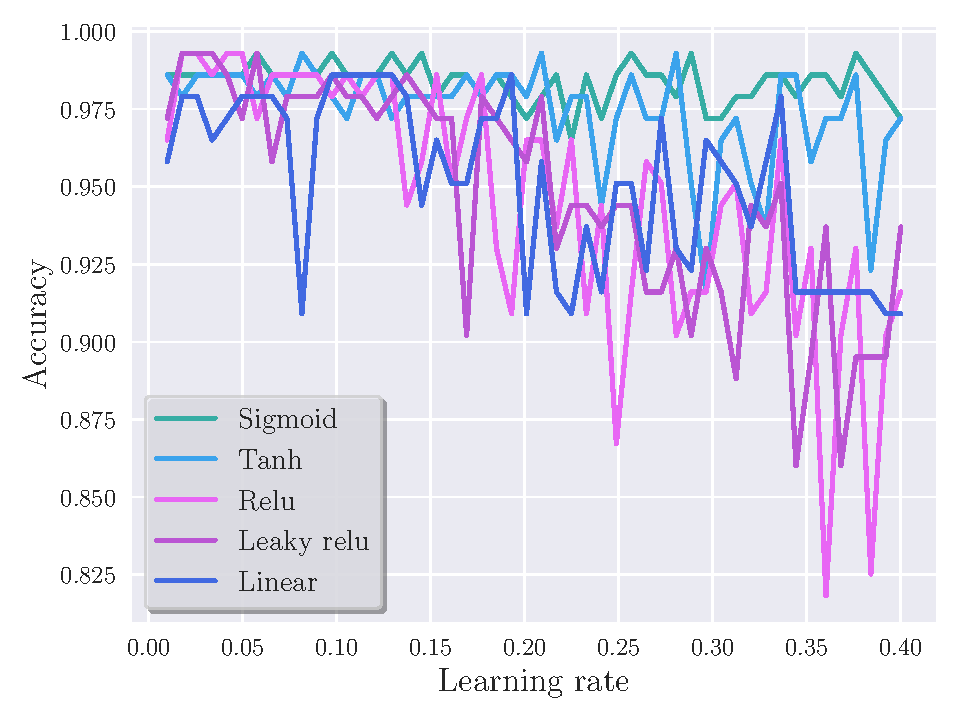
\includegraphics[width=\linewidth]{clasf_activation_functions2.pdf}
            \caption{$\eta \in [ 0.001, 0.01 ]$ with $n = 50$ points. One hidden layer 30 nodes}
            \label[fig]{res:fig:b}
        \end{subfigure}
        \hfill 
        \begin{subfigure}{.5\textwidth}
            \centering
            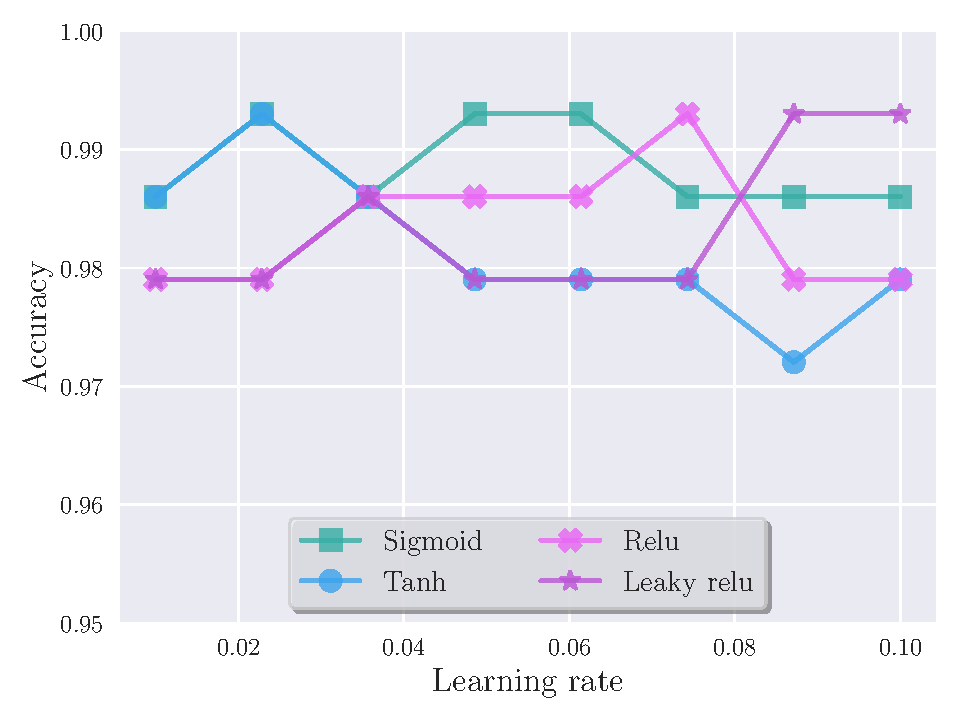
\includegraphics[width=\linewidth]{clasf_activation_functions3.pdf}
            \caption{$\eta \in [ 0.001, 0.01 ]$ with $n = 50$ points. Two hidden layers with 15 nodes each}
            \label[fig]{res:fig:c}
        \end{subfigure}
        \hfill 
        \begin{subfigure}{.5\textwidth}
            \centering
            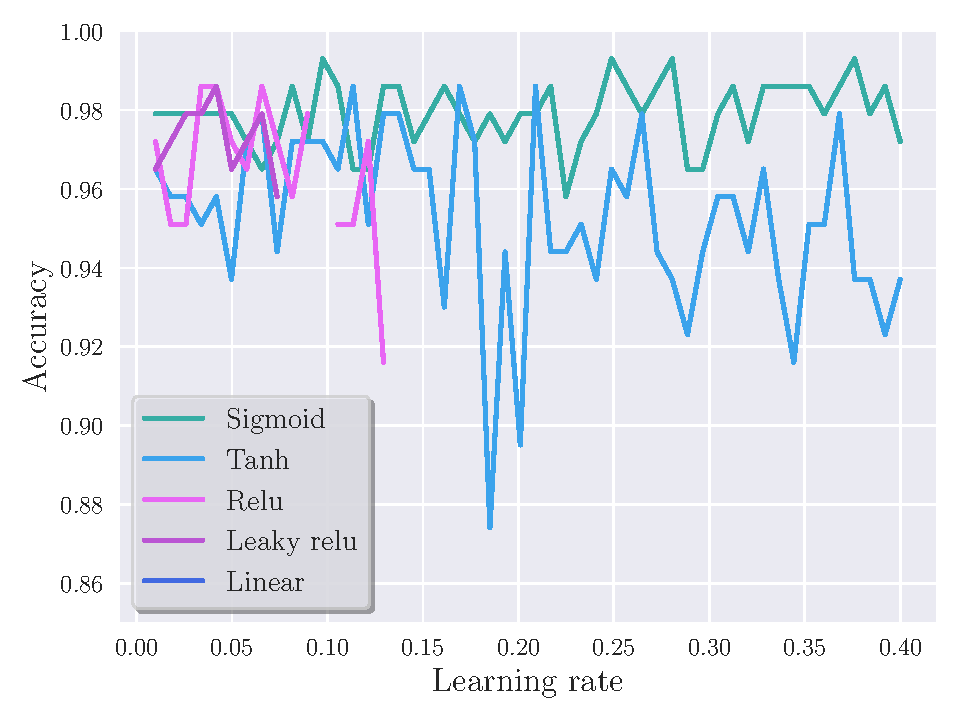
\includegraphics[width=\linewidth]{clasf_activation_functions4.pdf}
            \caption{$\eta \in [ 0.001, 0.01 ]$ with $n = 50$ points. Three hidden layers with ten nodes each}
            \label[fig]{res:fig:d}
        \end{subfigure}
    \end{figure*}